\section{GroupNode.h File Reference}
\label{GroupNode_8h}\index{GroupNode.h@{GroupNode.h}}


\subsection{Detailed Description}
\begin{Desc}
\item[Author:]Troy Taillefer \end{Desc}


\begin{Desc}
\item[Date:]December 7, 2007 \end{Desc}
\begin{Desc}
\item[Version:]0.1 \end{Desc}


Definition in file {\bf GroupNode.h}.

{\tt \#include \char`\"{}scenegraphnode.h\char`\"{}}\par


Include dependency graph for GroupNode.h:\nopagebreak
\begin{figure}[H]
\begin{center}
\leavevmode
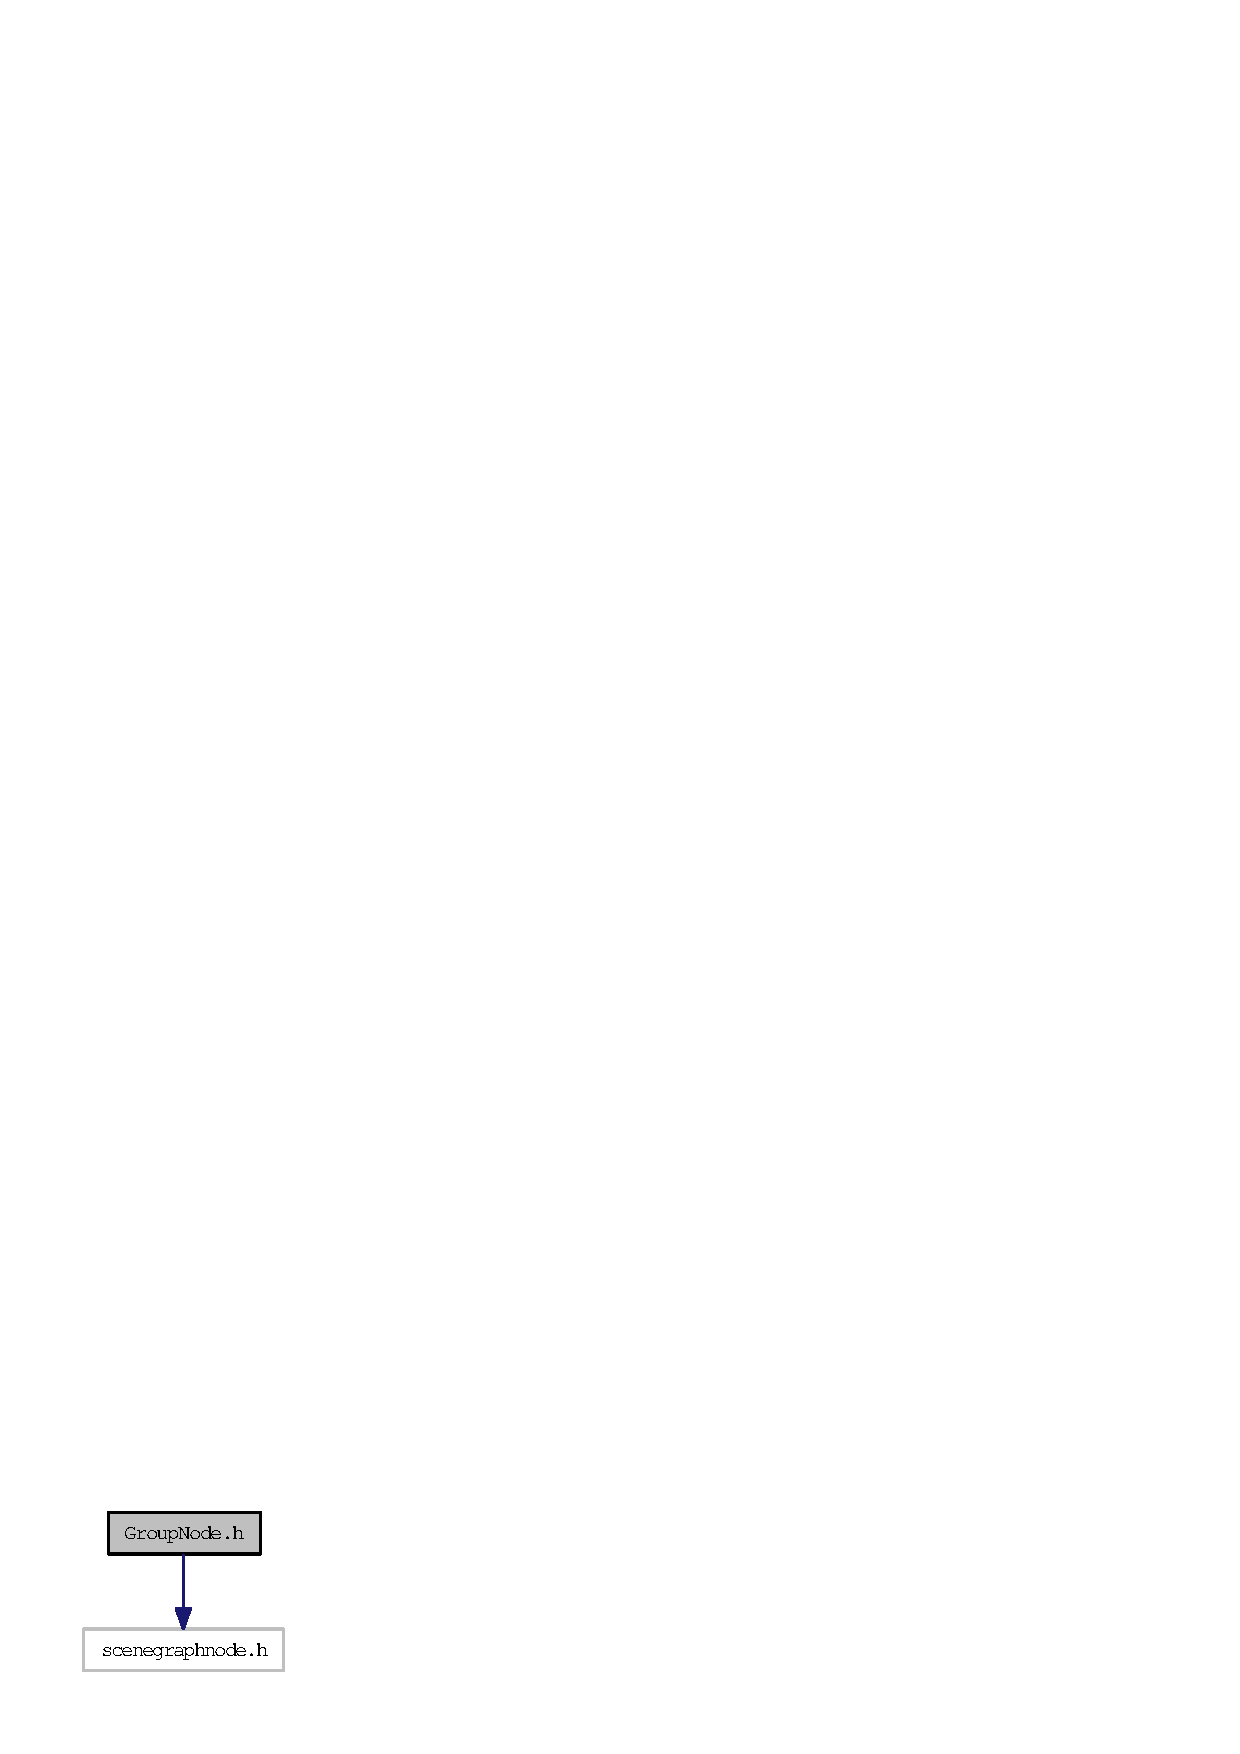
\includegraphics[width=70pt]{GroupNode_8h__incl}
\end{center}
\end{figure}


This graph shows which files directly or indirectly include this file:\nopagebreak
\begin{figure}[H]
\begin{center}
\leavevmode
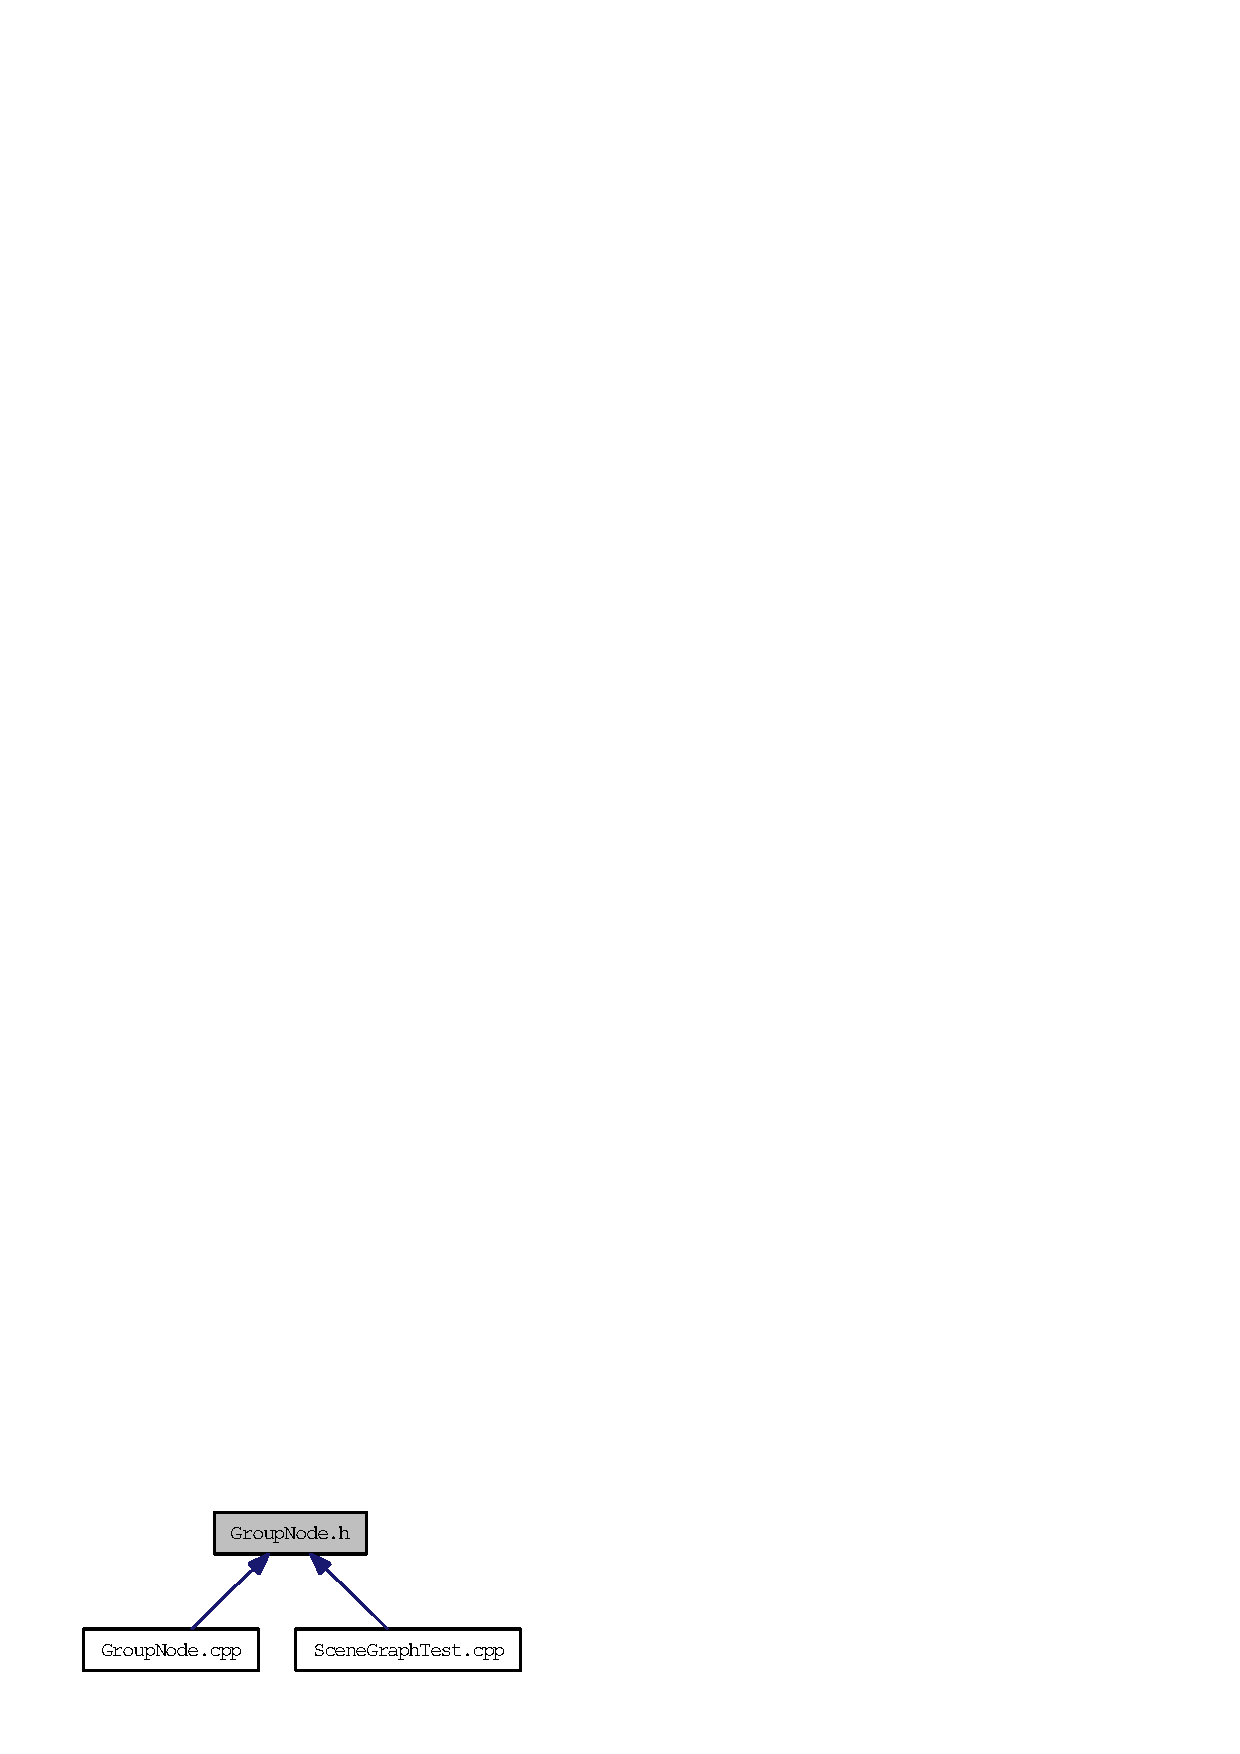
\includegraphics[width=127pt]{GroupNode_8h__dep__incl}
\end{center}
\end{figure}
\subsection*{Data Structures}
\begin{CompactItemize}
\item 
class {\bf GroupNode}
\begin{CompactList}\small\item\em This is a simple grouping node that is used to gather nodes together it implementation of setState and draw are the default empty it is node thats name captures the semantics of grouping other nodes. \item\end{CompactList}\end{CompactItemize}
